\PassOptionsToPackage{table,svgnames}{xcolor}
\PassOptionsToPackage{final}{graphicx}
\documentclass[sigconf,draft]{acmart}

\usepackage{booktabs} % For formal tables
\usepackage{graphicx}
\usepackage{subcaption}

\usepackage{todo}
\todoauthor[teal]{topa}

% Copyright
%\setcopyright{none}
%\setcopyright{acmcopyright}
\setcopyright{acmlicensed}
% \setcopyright{rightsretained}
%\setcopyright{usgov}
%\setcopyright{usgovmixed}
%\setcopyright{cagov}
%\setcopyright{cagovmixed}


% DOI
\acmDOI{10.475/123_4}

% ISBN
\acmISBN{123-4567-24-567/08/06}

%Conference
\acmConference[PX'17]{Programming Experience Workshop}{April 2017}{Brussels, Belgium} 
\acmYear{2017}
\copyrightyear{2017}

\acmPrice{15.00}


\begin{document}
\title{Smalltalk Debugger}
% \titlenote{}
\subtitle{Smalltalk-style Debugging Other Programming Languages}
% \subtitlenote{}


\author{Fabio Niephaus}
\affiliation{%
  \institution{Hasso Plattner Institute,\\University of Potsdam, Germany}
}
\email{fniephaus@acm.org}

\author{Tim Felgentreff}
\affiliation{%
  \institution{Hasso Plattner Institute,\\University of Potsdam, Germany}
}
\email{tim.felgentreff@hpi.de}

\author{Tobias Pape}
\affiliation{%
  \institution{Hasso Plattner Institute,\\University of Potsdam, Germany}
}
\email{tobias.pape@hpi.de}

\author{Robert Hirschfeld}
\affiliation{%
  \institution{Hasso Plattner Institute,\\University of Potsdam, Germany}
}
\email{robert.hirschfeld@hpi.de}


\begin{abstract}

\end{abstract}

%
% The code below should be generated by the tool at
% http://dl.acm.org/ccs.cfm
% Please copy and paste the code instead of the example below. 
%
\begin{CCSXML}
<ccs2012>
<concept>
<concept_id>10011007.10011006.10011066.10011069</concept_id>
<concept_desc>Software and its engineering~Integrated and visual development environments</concept_desc>
<concept_significance>300</concept_significance>
</concept>
<concept>
<concept_id>10011007.10011074.10011099.10011102.10011103</concept_id>
<concept_desc>Software and its engineering~Software testing and debugging</concept_desc>
<concept_significance>300</concept_significance>
</concept>
<concept>
<concept_id>10011007.10010940.10010941.10010942.10010948</concept_id>
<concept_desc>Software and its engineering~Virtual machines</concept_desc>
<concept_significance>100</concept_significance>
</concept>
</ccs2012>
\end{CCSXML}

\ccsdesc[300]{Software and its engineering~Integrated and visual development environments}
\ccsdesc[300]{Software and its engineering~Software testing and debugging}
\ccsdesc[100]{Software and its engineering~Virtual machines}

\keywords{Smalltalk, debugging, virtual machines}


\maketitle

\section{Background and Motivation}

\begin{figure}
  \centering
  \begin{subfigure}{.5\linewidth}
    \centering
    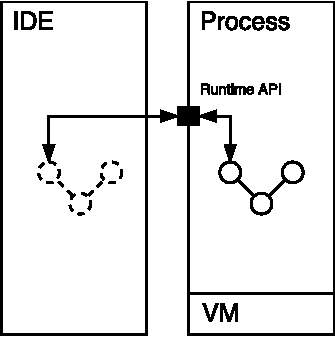
\includegraphics[width=.96\linewidth]{resources/ide_eclipse.pdf}
    \caption{Eclipse runs language in subprocess.}
    \label{fig:ide-eclipse}
  \end{subfigure}%
  \begin{subfigure}{.5\linewidth}
    \centering
    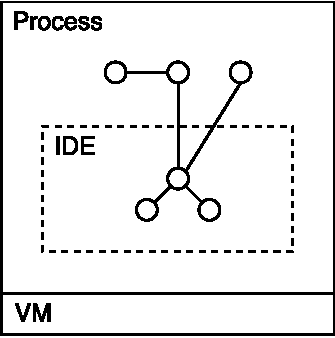
\includegraphics[width=.96\linewidth]{resources/ide_squeak.pdf}
    \caption{Squeak is part of the language process.}
    \label{fig:ide-squeak}
  \end{subfigure}
  \caption{Architectural comparison of Eclipse and Squeak.}
  \label{fig:ides}
\end{figure}

\todolist{JVM/CLR}{
\item JVM TI (JSR 163, \url{https://www.jcp.org/en/jsr/detail?id=163}) is readonly
\item \url{https://docs.oracle.com/javase/8/docs/platform/jvmti/jvmti.html}
\item Can only (a) force early return or (b) set local variable as intercession
\item CLR has dedicated, underdocumented Interface (\texttt{ICorDebug})
\item Edit-and-Continue anticipated but unavailable
  (\url{https://msdn.microsoft.com/en-us/library/ms231220(v=vs.110).aspx} says
  ``obsolete'')
\item Closest intercession: \texttt{ICorDebugEval}, executes arbitrary code, !Cumbersome!
  \url{https://blogs.msdn.microsoft.com/jmstall/2006/01/04/partition-of-icordebug/}
}

\section{Implementation}

\section{Evaluation}

\section{Conclusions}


\begin{acks}

\end{acks}

\bibliographystyle{ACM-Reference-Format}
\bibliography{sigproc} 

\end{document}

%%% Local Variables:
%%% mode: latex
%%% TeX-master: t
%%% TeX-engine: luatex
%%% End:
